\documentclass[11pt,a4paper]{article}

\bibliographystyle{ieeetr}

\usepackage[margin=1in]{geometry}
\usepackage{graphicx}
\usepackage{subfig}
\usepackage{amsmath}
\usepackage{url}

\title{Cellular Automata and Computational Universality}

\begin{document}

\maketitle

\begin{center}
    Thomas Archbold \\
    University of Warwick \\
    \texttt{T.Archbold@warwick.ac.uk}
\end{center}

\begin{abstract}
    Cellular automata are discrete models with the ability to not only give rise
    to beautiful, intricate patterns, but also to be used as powerful tools of
    computation, with applications in cryptography, error-correction coding, and
    simulation of computer processors, to name a few. They also raise profound
    questions about the nature of our reality, asking whether our universe could
    be one such automaton. This paper provides a discussion into these automata,
    exploring the various power and limitations of a number of specific rule
    sets, covering John Conway's well-known ``Game of Life'' to the more obscure
    ``Langton's ant'' and ``Wireworld''. In particular, it explores the notion
    of computational universality, or Turing completeness, an automaton's
    ability to simulate any conceivable computation, and considers their
    potential in the context of solving two specific problems, the Firing Squad
    Synchronisation Problem and the Majority Problem. Existing solutions to
    these problems are explored, and their existing avenues for optimisation are
    discussed. In order to fully appreciate the complex structures that can
    arise from such simple beginnings, this project also presents software to
    visualise and probe further into the nature of the automata highlighted.
\end{abstract}

\section{Introduction}
    A cellular automaton is a discrete model of computation which consists of a
    finite collection of ``cells'', each in one of a finite number of states.
    The state of each of these cells may evolve over the discrete progression of
    time in discrete steps, and may do so according to a deterministic set of
    rules specifying the state to which each cell is to progress, taking into
    account the states of cells in its neighbourhood. Their inherently discrete
    nature allows for strong analogies to be made with digital computers, and
    gifts them the ability to simulate digital processes and the potential to
    solve problems in this area. 
    
    Consider the cellular automaton defined by the simple rule:
    \begin{equation}
        \label{rule90}
        a_{i}^{t+1} = a_{i-1}^{t} + a_{i+1}^{t} \mod{2}
    \end{equation}

    For any automaton, in each time step the rule is applied to all cells in the
    automaton instantaneously and simultaneously. In this case, our set of
    states is ${0,1}$, and for each cell we look at the cells immediately
    preceding and succeeding it: if exactly one of them is in state 1, then this
    cell will be in state 1 in the next time step. Otherwise it will be in state
    0.

    \begin{figure}[h]
        \begin{center}
            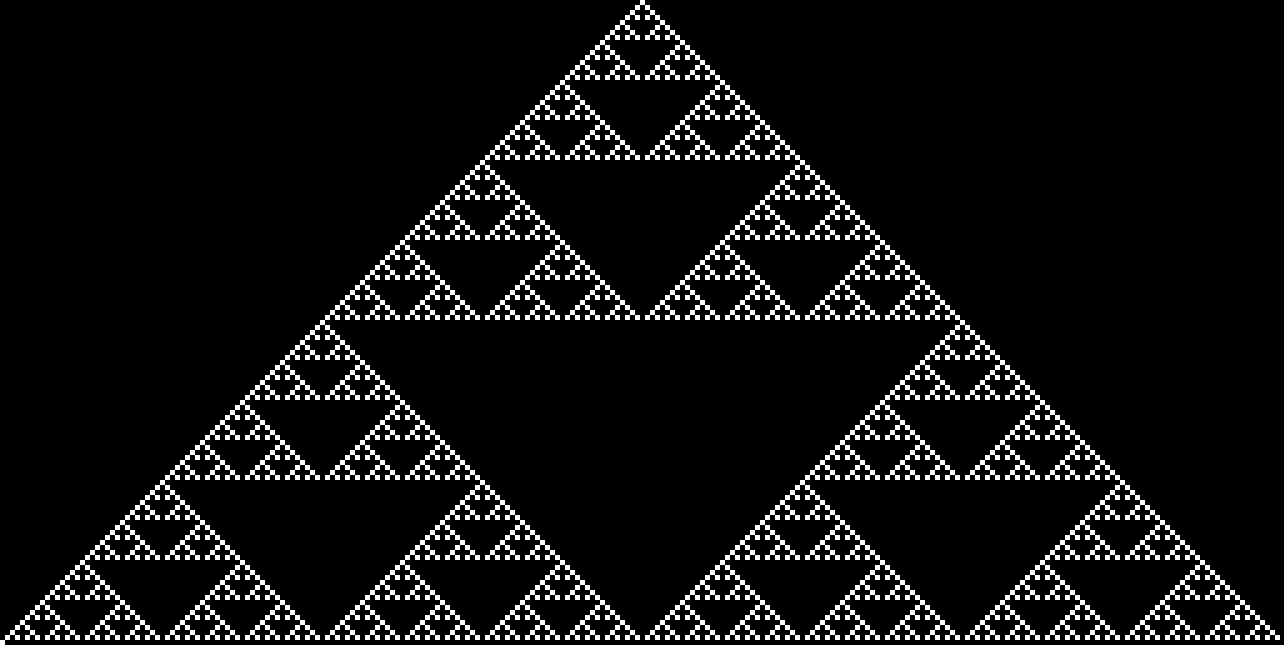
\includegraphics[width=4in]{rule1.png}
            \caption{Pattern generated from applying Eq. 1 over 129 generations}
            \label{fig:rule90}
        \end{center}
    \end{figure}

    \subsection{Self-similarity}
    Figure \ref{fig:rule90} shows a visualisation of Eq. \ref{rule90}. A cell is
    filled white if it has the value 1, and black otherwise. Note that each new
    ``line'' of the visualisation represents the automaton in the next
    successive time-step from the one before; this automaton is one-dimensional,
    and so we may represent it in its entirety as a single row of cells. This
    pattern exhibits two important characteristics, the first of which is
    ``self-similarity'', meaning that portions of the pattern generated are
    indistinguishable from the whole when magnified. As Wolfram states, in this
    way ``the pattern is therefore invariant under rescaling... and may be
    characterised by a fractal dimension''\cite{WolframFractal}. One such
    definition of this is the Hausdorff-Besicovitch dimension\cite{Hausdorff}.

    As an example, suppose we have a cube with some mass, and we wish to find
    out how the mass scales when we try to make the same cube out of smaller
    copies of the original. Intuitively, one way to do this require eight
    smaller cubes, each of whose side length is half that of the original cube.
    So with the scaling factor of $\frac{1}{2}$, the mass of each smaller cube
    is $\frac{1}{8} = (\frac{1}{2})^3$.
    So we arrive at the equation $N = S^D$, where $N$ is the number of smaller
    copies that can be stuck together to make the original, $S$ is the scaling
    factor of these smaller copies, and $D$ is the dimension. In this example, we
    compute that the dimension of a cube is 3, which is obviously correct.  Back
    to the dimension of the Sierpinski Triangle, we can see that each larger
    triangle is made up of three smaller triangles, each of whose side lengths
    are half that of the larger triangle. So we calculate the dimension as:

    \begin{equation}
        \label{sierpinskiDim}
        \begin{split}
            \tfrac{1}{3} & = (\tfrac{1}{2})^D \\
            \log{\tfrac{1}{3}} &= D \log{\tfrac{1}{2}} \\
            D &= \tfrac{\log{3}}{\log{2}} \approx 1.585
        \end{split}
    \end{equation}

    Many naturally-occurring systems exhibit fractal structures, from snowflakes
    to pine cones to Romanesco broccoli, and raises the possibility that these
    are generated through the evolution of some natural cellular automata or
    similar processes.

    \begin{figure}[h]%
        \centering
        \subfloat[Snowflake]{{\includegraphics[width=5cm]{snowflake.jpg}}}%
        \qquad
        \subfloat[Romanesco broccoli]{{\includegraphics[width=5cm]{romanesco_broccoli.jpg}}}%
        \caption{Snowflakes and Romanesco broccoli exhibit fractal structures}%
        \label{fig:nature_fractals}%
    \end{figure}

    \subsection{Self-organisation}
    Second of the characteristics exhibited by this cellular automaton is
    ``self-organisation'', 

\section{}
\section{Examples}
\section{Applications}
\section{Computational Universality}
\section{Firing Squad Synchronisation Problem}
\section{Majority Problem}
\section{}

\bibliography{bibliography}

\end{document}
